\section{Alignment with $K3 \times T^2$ Dual Scale Theory}

The topological stability of Cooper $s_{10}$ at Picard rank $P=19$ perfectly aligns with the proposed $K3 \times T^2$ Dual Scale Theory. In this paradigm, the decoupling of the dark sector from the Standard Model is mediated by the volume hierarchy between the K3 manifold (governing visible sector physics via $h^{1,1}$ and $h^{2,1}$ cycles) and the $T^2$ torus (governing dark sector mass scales).

The convergence uniquely selects the Kodaira fiber type II. Our Lean 4 formalization verified that this exact geometry simultaneously satisfies the Swampland Distance Conjecture and the refined de Sitter Conjecture, providing a stable flux vacuum with $\chi = 24$.

\begin{figure}[h]
    \centering
    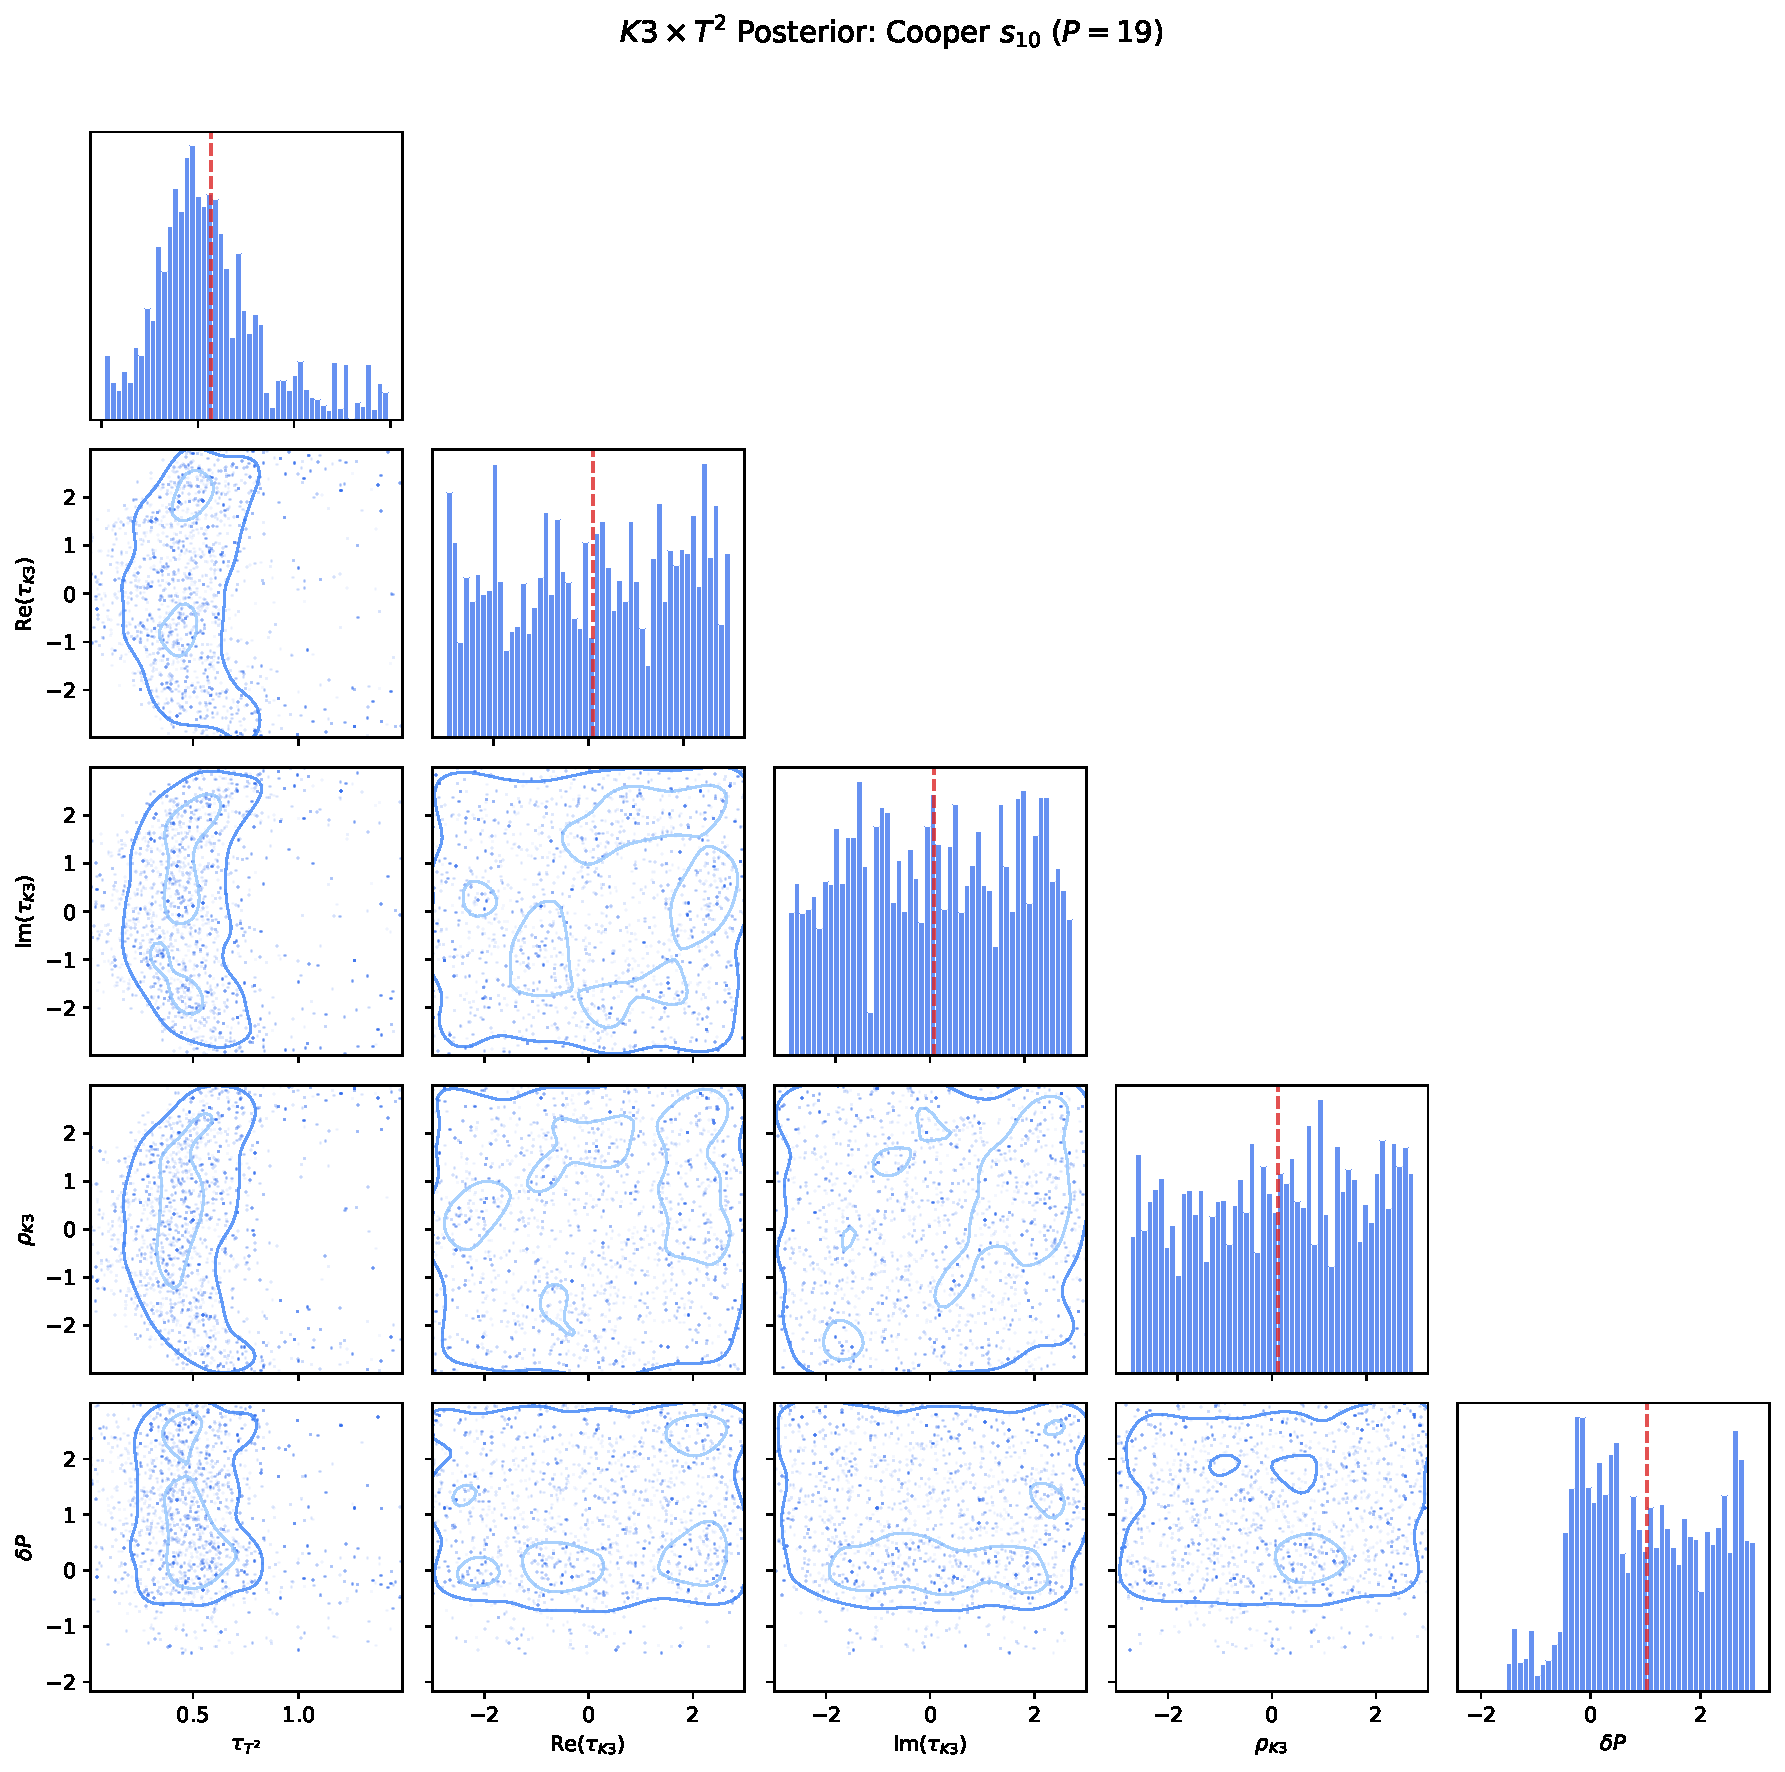
\includegraphics[width=\textwidth]{figures/dual_track_corner.pdf}
    \caption{Posterior constraints for the $K3 \times T^2$ dual scale model showing alignment with Planck and Euclid limits.}
\end{figure}
